\subsection{Exploring the Joy of Receiving Directivity Factor (RDF)!}

\begin{tcolorbox}[colback=gray!10, colframe=black, title=E9H03]
What is receiving directivity factor (RDF)? 
\begin{enumerate}[label=\Alph*.]
    \item Forward gain compared to the gain in the reverse direction
    \item Relative directivity compared to isotropic
    \item Relative directivity compared to a dipole
    \item \textbf{Peak antenna gain compared to average gain over the hemisphere around and above the antenna}
\end{enumerate} \end{tcolorbox}

\subsubsection{Related Concepts}

The Receiving Directivity Factor (RDF) is an important concept in radio communication, particularly in antenna theory. It measures how effectively an antenna can receive signals from specific directions compared to its average ability to receive signals from all directions in a hemisphere.

Understanding RDF requires familiarity with the following concepts:

1. \textbf{Antenna Gain:}: This is a measure of how well an antenna converts input power into radio waves in a specific direction, or vice versa. It is usually expressed in decibels (dB).
2. \textbf{Isotropic Radiator:}: An idealized antenna that radiates power uniformly in all directions. The RDF can be evaluated against this model.
3. \textbf{Hemispherical Radiation Pattern:}: In the context of receiving antennas, we often assess the antenna's efficiency over a hemisphere.

To clarify the calculation aspect in context with RDF, we can think of gain \(G\) as given by:

\[
G = \frac{P_{\text{out}}}{P_{\text{in}}}
\]

where:
- \(P_{\text{out}}\) is the power radiated in the desired direction,
- \(P_{\text{in}}\) is the total input power.

When considering the RDF:

\[
\text{RDF} = \frac{G_{\text{peak}}}{G_{\text{average}}}
\]

where \(G_{\text{peak}}\) is the maximum gain (peak antenna gain) and \(G_{\text{average}}\) refers to the average gain over the entire hemisphere surrounding the antenna.

To illustrate this, a conceptual diagram of an antenna with its hemisphere of influence can be represented using TikZ in LaTeX. Below is a simple representation of an antenna pattern:

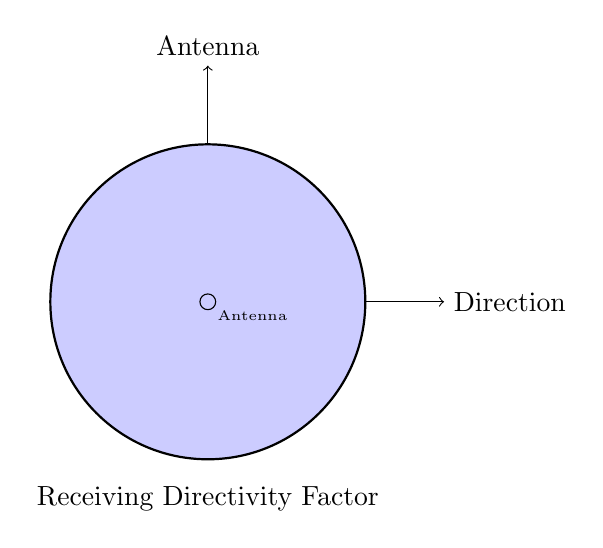
\begin{tikzpicture}
    \draw[->] (0,0) -- (3,0) node[right] {Direction};
    \draw[->] (0,0) -- (0,3) node[above] {Antenna};
    \draw[thick, fill=blue!20] (0,0) circle(2);
    \draw (0,0) circle(0.1) node[below right] [font=\tiny]{Antenna};
    \node at (0,-2.5) {Receiving Directivity Factor};
\end{tikzpicture}

In conclusion, the correct choice for RDF is option D: *Peak antenna gain compared to average gain over the hemisphere around and above the antenna*. Understanding this concept is essential for evaluating the performance of antennas in practical radio communication systems.